\documentclass[letterpaper, 12pt]{article}

\usepackage{amsmath}
\usepackage{amssymb}
\usepackage{pgfplots}

\title{Probability and Statistics}
\author{Alvin Lin}
\date{Probability and Statistics: January 2017 - May 2017}

\begin{document}

\maketitle

\section{Inferential Statistics}
Suppose there is a set of people who can vote and a subset of them
whom we want to survey. We can make a prediction about the people
who can vote by surveying the subset. The set of people who can
vote is called a \textbf{population} and the set of people surveyed
is called a \textbf{sample}. This is known as inferential statistics.
\[ population \to sample \quad \mathrm{(Probability)} \]
\[ sample \gets population \quad \mathrm{(Inferential\ statistics)} \]

Consider the experiment of tossing a coin twice. The
\textbf{sample space} of this experiment is the set
\[ \bigg\{ (H,H), (H,T), (T,H), (T,T) \bigg\} \]
Each element (e.g. (T,H)) is a sample point.

\subsection{Example Problem}
For each of the following hypothetical populations, give a plausible
sample of size 4.

All distances that might result when you throw a football (feet):
\[ \bigg\{ 32, 40, 50, 46 \bigg\} \]

Page lengths of books published 5 years from now:
\[ \bigg\{ 520, 600, 670, 700 \bigg\} \]

\section{Descriptive Statistics}
In descriptive statistics, we do not make predictions. We use tools such
as mean, median, and mode to describe data, and visualizations such as
histograms and box plots.

\subsection{Example Problem}
Suppose we have 20 one-quart water bottles and of those 20, we select 5
water bottles. The pH values of water in the 20 water bottles is the
population and the ph value of water in the 5 selected bottles is the sample.

The sample size is 5 \( (n = 5) \). We can use the variable \( x \) to denote
pH values. Individual observations can be denoted \( x_{1}, x_{2}, x_{3}, x_{4},
x_{5} \).

Suppose the range of the function x is
\( \big\{ 6.1, 6.8, 6.8, 7.1, 7.4 \big\} \).

The frequency of 6.1 is 1. \par
The frequency of 6.8 is 2. \par
The frequency of 9.0 is 0. \par
The relative frequency of 6.1 is \( \frac{1}{5} = 0.2 = 20\% \). \par
The relative frequency of 6.8 is \( \frac{2}{5} = 0.4 = 40\% \).

\begin{center}
  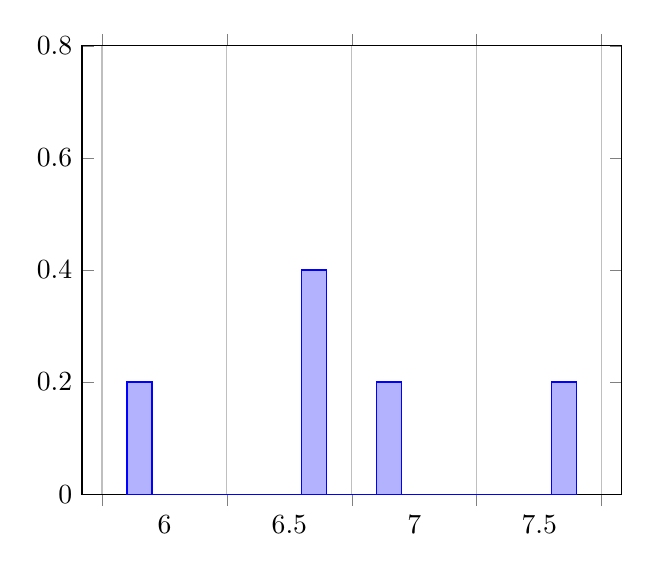
\begin{tikzpicture}
    \begin{axis}[
      ybar interval,
      ymax=0.8,
      ymin=0,
      xtick={6,6.5,7,7.5,8}
    ]
    \addplot coordinates {
      (6.1,0.2) (6.2,-1)
      (6.8,0.4) (6.9,-1)
      (7.1,0.2) (7.2,-1)
      (7.8,0.2) (7.9,-1)
    };
    \end{axis}
  \end{tikzpicture}
\end{center}

\subsection{Countable and Uncountable Sets}
\begin{align*}
  Let: A &= \bigg\{ 1, 2, 3, 4, 5 \bigg\} \\
  B &= \bigg\{ 0.0, 0.1, 0.2, 0.3, \dots, 13.9, 14.0 \bigg\} \\
  C &= \bigg[ 0, 14 \bigg] \\
\end{align*}
If we represent the function \( x \) as:
\[ \bigg\{ x \mid A \to B \bigg\} \]
B is a countable set and x is a discrete variable.
If we represent the function \( x \) as:
\[ \bigg\{ x \mid A \to C \bigg\} \]
C is a countable set and x is a continuous variable.
Set theory can be applied to functions of the following type:
\[ f:A \to C \subseteq \mathbb{R} \]

Let \( W = \big\{ 0, 1, 2, 3, \dots \big\} \). A set \( A \) is called
countable if there is a bijective (one-to-one) function from \( A \) to a
subset of \( W \). Otherwise, \( A \) is uncountable.
Countable sets:
\[ \bigg\{ James, Tina, Christine \bigg\} \]
\[ \bigg\{ 1, 8, 13, 17 \bigg\} \]
\[ \bigg\{ 1, \frac{1}{2}, \frac{1}{3}, \frac{1}{4}, \dots \bigg\} \]
\[ \bigg\{ \dots, -3, -2, -1, 0, 1, 2, 3, \dots \bigg\} \]
Uncountable sets:
\[ \bigg[ 0, 1 \bigg] \]
\[ \bigg( 0, 1 \bigg] \]
\[ \bigg( 0, 1 \bigg) \]
\[ \mathbb{R} \]

\subsection{Power set of a set}
A power set of \( A \), \( P(A) \mathrm{\ or\ } 2^{A} \), is the set containing
all subsets of A.
\[ Let: A = \bigg\{ 1, 2, 3 \bigg\} \]
\[ 2^{A} = \bigg\{ \emptyset, 1, 2, 3, \{1, 2\}, \{1, 3\}, \{2, 3\},
   \{1, 2, 3\} \bigg\} \]

\end{document}
